\documentclass[tikz]{standalone}
% \usepackage{tikz} % already loaded by the documentclass


\begin{document}
%%| filename: forword-backword
%%| caption: Backpropagation
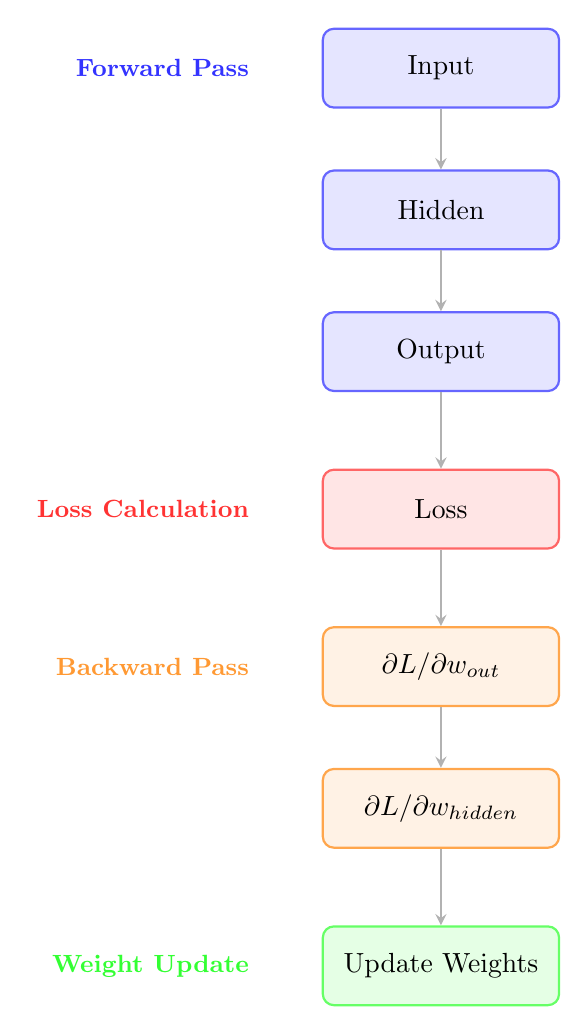
\begin{tikzpicture}[
    node distance=1.8cm,
    block/.style={
        rectangle,
        draw=black!80,
        fill=white,
        thick,
        rounded corners=4pt,
        minimum width=3cm,
        minimum height=1cm,
        align=center
    },
    forward/.style={
        block,
        fill=blue!10,
        draw=blue!60
    },
    loss/.style={
        block,
        fill=red!10,
        draw=red!60
    },
    backward/.style={
        block,
        fill=orange!10,
        draw=orange!70
    },
    update/.style={
        block,
        fill=green!10,
        draw=green!60
    },
    arrow/.style={
        ->,
        >=stealth,
        thick,
        gray!60
    }
]

\usetikzlibrary{calc}

% --- Forward Pass (vertical stack) ---
\node[forward] (A) {Input};
\node[forward, below of=A] (B) {Hidden};
\node[forward, below of=B] (C) {Output};

\draw[arrow] (A) -- (B);
\draw[arrow] (B) -- (C);

% --- Loss Calculation ---
\node[loss, below of=C, node distance=2cm] (D) {Loss};

\draw[arrow] (C) -- (D);

% --- Backward Pass (vertical stack) ---
\node[backward, below of=D, node distance=2cm] (E) {$\partial L / \partial w_{out}$};
\node[backward, below of=E] (F) {$\partial L / \partial w_{hidden}$};

\draw[arrow] (D) -- (E);
\draw[arrow] (E) -- (F);

% --- Weight Update ---
\node[update, below of=F, node distance=2cm] (G) {Update Weights};

\draw[arrow] (F) -- (G);

% --- Subgraph labels (positionnées à gauche des blocs) ---
\node[font=\small\bfseries, text=blue!80, anchor=east] at ($(A.west)+(-0.8,0)$) {Forward Pass};
\node[font=\small\bfseries, text=red!80, anchor=east] at ($(D.west)+(-0.8,0)$) {Loss Calculation};
\node[font=\small\bfseries, text=orange!80, anchor=east] at ($(E.west)+(-0.8,0)$) {Backward Pass};
\node[font=\small\bfseries, text=green!80, anchor=east] at ($(G.west)+(-0.8,0)$) {Weight Update};

\end{tikzpicture}
\end{document}
      